\documentclass[CJK]{beamer}
\usepackage{CJKutf8}
\usepackage{beamerthemesplit}
\usetheme{Malmoe}
\useoutertheme[footline=authortitle]{miniframes}
\usepackage{amsmath}
\usepackage{amssymb}
\usepackage{graphicx}
\usepackage{eufrak}
\usepackage{color}
\usepackage{slashed}
\usepackage{simplewick}
\usepackage{tikz}
\usepackage{tcolorbox}
\graphicspath{{../figures/}}
%%figures
\def\lfig#1#2{\includegraphics[width=#1 in]{#2}}
\def\addfig#1#2{\begin{center}\includegraphics[width=#1 in]{#2}\end{center}}
\def\wulian{
\includegraphics[width=0.18in]{emoji_wulian.jpg}}
\def\bigwulian{
\includegraphics[width=0.35in]{emoji_wulian.jpg}}
\def\bye{
\includegraphics[width=0.18in]{emoji_bye.jpg}}
\def\bigbye{
\includegraphics[width=0.35in]{emoji_bye.jpg}}
\def\huaixiao{
\includegraphics[width=0.18in]{emoji_huaixiao.jpg}}
\def\bighuaixiao{
\includegraphics[width=0.35in]{emoji_huaixiao.jpg}}
%% colors
\def\blacktext#1{{\color{black}#1}}
\def\bluetext#1{{\color{blue}#1}}
\def\redtext#1{{\color{red}#1}}
\def\darkbluetext#1{{\color[rgb]{0,0.2,0.6}#1}}
\def\skybluetext#1{{\color[rgb]{0.2,0.7,1.}#1}}
\def\cyantext#1{{\color[rgb]{0.,0.5,0.5}#1}}
\def\greentext#1{{\color[rgb]{0,0.7,0.1}#1}}
\def\darkgray{\color[rgb]{0.2,0.2,0.2}}
\def\lightgray{\color[rgb]{0.6,0.6,0.6}}
\def\gray{\color[rgb]{0.4,0.4,0.4}}
\def\blue{\color{blue}}
\def\red{\color{red}}
\def\green{\color{green}}
\def\darkgreen{\color[rgb]{0,0.4,0.1}}
\def\darkblue{\color[rgb]{0,0.2,0.6}}
\def\skyblue{\color[rgb]{0.2,0.7,1.}}
%%control
\def\be{\begin{equation}}
\def\ee{\nonumber\end{equation}}
\def\bea{\begin{eqnarray}}
\def\eea{\nonumber\end{eqnarray}}
\def\bch{\begin{CJK}{UTF8}{gbsn}}
\def\ech{\end{CJK}}
\def\bitem{\begin{itemize}}
\def\eitem{\end{itemize}}
\def\bcenter{\begin{center}}
\def\ecenter{\end{center}}
\def\bex{\begin{minipage}{0.2\textwidth}
\includegraphics[width=0.6in]{jugelizi.png}\end{minipage}\begin{minipage}{0.76\textwidth}}
\def\eex{\end{minipage}}
\def\chtitle#1{\frametitle{\bch#1\ech}}
\def\bmat#1{\left(\begin{array}{#1}}
\def\emat{\end{array}\right)}
\def\bcase#1{\left\{\begin{array}{#1}}
\def\ecase{\end{array}\right.}
\def\bmini#1{\begin{minipage}{#1\textwidth}}
\def\emini{\end{minipage}}
\def\tbox#1{\begin{tcolorbox}#1\end{tcolorbox}}
\def\pfrac#1#2#3{\left(\frac{\partial #1}{\partial #2}\right)_{#3}}
%%symbols
\def\sone{$\star$}
\def\stwo{$\star\star$}
\def\sthree{$\star\star\star$}
\def\sfour{$\star\star\star\star$}
\def\sfive{$\star\star\star\star\star$}
\def\rint{{\int_\leftrightarrow}}
\def\roint{{\oint_\leftrightarrow}}
\def\stdHf{{\textit{\r H}_f}}
\def\deltaH{{\Delta \textit{\r H}}}
\def\ii{{\dot{\imath}}}
\def\skipline{{\vskip0.1in}}
\def\skiplines{{\vskip0.2in}}
\def\lagr{{\mathcal{L}}}
\def\hamil{{\mathcal{H}}}
\def\vecv{{\mathbf{v}}}
\def\vecx{{\mathbf{x}}}
\def\vecy{{\mathbf{y}}}
\def\veck{{\mathbf{k}}}
\def\vecp{{\mathbf{p}}}
\def\vecn{{\mathbf{n}}}
\def\vecA{{\mathbf{A}}}
\def\vecP{{\mathbf{P}}}
\def\vecsigma{{\mathbf{\sigma}}}
\def\hatJn{{\hat{J_\vecn}}}
\def\hatJx{{\hat{J_x}}}
\def\hatJy{{\hat{J_y}}}
\def\hatJz{{\hat{J_z}}}
\def\hatj#1{\hat{J_{#1}}}
\def\hatphi{{\hat{\phi}}}
\def\hatq{{\hat{q}}}
\def\hatpi{{\hat{\pi}}}
\def\vel{\upsilon}
\def\Dint{{\mathcal{D}}}
\def\adag{{\hat{a}^\dagger}}
\def\bdag{{\hat{b}^\dagger}}
\def\cdag{{\hat{c}^\dagger}}
\def\ddag{{\hat{d}^\dagger}}
\def\hata{{\hat{a}}}
\def\hatb{{\hat{b}}}
\def\hatc{{\hat{c}}}
\def\hatd{{\hat{d}}}
\def\hatN{{\hat{N}}}
\def\hatH{{\hat{H}}}
\def\hatp{{\hat{p}}}
\def\Fup{{F^{\mu\nu}}}
\def\Fdown{{F_{\mu\nu}}}
\def\newl{\nonumber \\}
\def\vece{\mathrm{e}}
\def\calM{{\mathcal{M}}}
\def\calT{{\mathcal{T}}}
\def\calR{{\mathcal{R}}}
\def\barpsi{\bar{\psi}}
\def\baru{\bar{u}}
\def\barv{\bar{\upsilon}}
\def\qeq{\stackrel{?}{=}}
\def\torder#1{\mathcal{T}\left(#1\right)}
\def\rorder#1{\mathcal{R}\left(#1\right)}
\def\contr#1#2{\contraction{}{#1}{}{#2}#1#2}
\def\trof#1{\mathrm{Tr}\left(#1\right)}
\def\trace{\mathrm{Tr}}
\def\comm#1{\ \ \ \left(\mathrm{used}\ #1\right)}
\def\tcomm#1{\ \ \ (\text{#1})}
\def\slp{\slashed{p}}
\def\slk{\slashed{k}}
\def\calp{{\mathfrak{p}}}
\def\veccalp{\mathbf{\mathfrak{p}}}
\def\Tthree{T_{\tiny \textcircled{3}}}
\def\pthree{p_{\tiny \textcircled{3}}}
\def\dbar{{\,\mathchar'26\mkern-12mu d}}
\def\erf{\mathrm{erf}}
\def\const{\mathrm{constant}}
\def\pheat{\pfrac p{\ln T}V}
\def\vheat{\pfrac V{\ln T}p}
%%units
\def\fdeg{{^\circ \mathrm{F}}}
\def\cdeg{^\circ \mathrm{C}}
\def\atm{\,\mathrm{atm}}
\def\angstrom{\,\text{\AA}}
\def\SIL{\,\mathrm{L}}
\def\SIkm{\,\mathrm{km}}
\def\SIyr{\,\mathrm{yr}}
\def\SIGyr{\,\mathrm{Gyr}}
\def\SIV{\,\mathrm{V}}
\def\SImV{\,\mathrm{mV}}
\def\SIeV{\,\mathrm{eV}}
\def\SIkeV{\,\mathrm{keV}}
\def\SIMeV{\,\mathrm{MeV}}
\def\SIGeV{\,\mathrm{GeV}}
\def\SIcal{\,\mathrm{cal}}
\def\SIkcal{\,\mathrm{kcal}}
\def\SImol{\,\mathrm{mol}}
\def\SIN{\,\mathrm{N}}
\def\SIHz{\,\mathrm{Hz}}
\def\SIm{\,\mathrm{m}}
\def\SIcm{\,\mathrm{cm}}
\def\SIfm{\,\mathrm{fm}}
\def\SImm{\,\mathrm{mm}}
\def\SInm{\,\mathrm{nm}}
\def\SImum{\,\mathrm{\mu m}}
\def\SIJ{\,\mathrm{J}}
\def\SIW{\,\mathrm{W}}
\def\SIkJ{\,\mathrm{kJ}}
\def\SIs{\,\mathrm{s}}
\def\SIkg{\,\mathrm{kg}}
\def\SIg{\,\mathrm{g}}
\def\SIK{\,\mathrm{K}}
\def\SImmHg{\,\mathrm{mmHg}}
\def\SIPa{\,\mathrm{Pa}}

\def\courseurl{https://github.com/zqhuang/SYSU\_TD}

\def\tpage#1#2{
\begin{frame}
\begin{center}
\begin{Large}
\bch
热学 \\
第#1讲 #2

{\vskip 0.3in}

黄志琦

\ech
\end{Large}
\end{center}

\vskip 0.2in

\bch
教材:《热学》第二版,赵凯华,罗蔚茵,高等教育出版社
\ech

\bch
课件下载
\ech
\courseurl
\end{frame}
}

\title{Lesson 02 - Heat and State}
  \author{}
  \date{}
\begin{document}
\tpage{2}{热量与物态}

\begin{frame}
\bch
今天的内容比较乱,请做好风中凌乱的准备…
\ech
\end{frame}

\begin{frame}
\chtitle{热量是能量的一种形式}
\bch
\bitem
\item{既然组成物体的微观粒子(为了叙述简单,以下我们统称分子,实际上这些粒子可以是原子甚至其他更基本的粒子)可以带有能量,那么物体就有一个“内能”。{\bf 内能不仅包括分子的动能,还包括由分子之间的分子力而产生的势能。}}
\item{\bf 加热是传递能量给该物体,改变它存储的内能。}
\item{历史上习惯用的热量单位是“卡”(cal),最初定义是在$1\atm$下使$1\SIg$纯水从$14.5\cdeg$升高到$15.5\cdeg$时需要的热量。日常环境下这个量对压强和温度的依赖并不敏感,我们往往{\bf 粗略地说1卡就是日常条件下$1\SIg$水升温$1\cdeg$需要的热量。}}
\item{热量只是能量的一种形式,经实验测定 $1\SIcal \approx 4.2\SIJ$。后来$\SIcal$重新按下式进行了{\bf 定义}:
$$1\SIcal = 4.184 \SIJ$$
普适气体常量$R$的值用卡来写比较简洁,大约为$2\SIcal/(\SImol\cdot\SIK)$。}
\eitem

\ech
\end{frame}

\begin{frame}
\chtitle{思考题}
\bch
一个$60\SIkg$的成年人日常需要消耗大约1500大卡(就是千卡,$\SIkcal$)的热量来维持身体机能,试计算这些能量能够把他举高到多少米?
\ech
\end{frame}



\begin{frame}
\chtitle{热容量(Heat Capacity)和比热容(Specific Heat Capacity)}
\bch
\bitem
\item{物质温度升高(降低)$1\SIK$时所吸收(放出)的热量,代表了该物质存储热量的能力,我们称之为称为{\bf 热容量},通常用大写$C$来表示。}
\item{{\bf 单位质量物质的热容量称为 比热容},或简称比热,通常用小写$c$来表示。撇开对环境的弱依赖性不谈,我们可粗略地说水的比热容是$4190\SIJ/(\SIkg\cdot\SIK)$,水银的比热容是$139\SIJ/(\SIkg\cdot\SIK)$, 铝的比热容是$900\SIJ/(\SIkg\cdot\SIK)$,等等。}
\item{在常见物质中,水的比热几乎是最大的。}
\item{我们也可以定义每$\SImol$物质的热容量为摩尔热容(记为$C^{\SImol}$),了解即可,在本课就不多做介绍了。}
\eitem
\ech
\end{frame}


\begin{frame}
\chtitle{思考题}
\bch
\bcenter
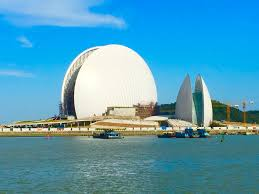
\includegraphics[width=1.in]{zhuhai.jpg}
\ecenter

为什么靠近海边的地方(例如珠海)温度变化范围小?
\ech
\end{frame}


\begin{frame}
\chtitle{思考题}
\bch
加热一定使物体的温度升高吗?
\ech
\end{frame}


\begin{frame}
\chtitle{加了热不一定变更热(\wulian我怀疑我加了假热)}
\bch
\bitem
\item{虽然加热的本质是传递能量给物体使物体内能增大,但物体的内能包含了分子的动能和势能,原则上来讲,传递的能量可以都用来改变势能,分子平均动能未必一定会增大,所以温度未必会升高。}
\eitem

\skipline

\wulian只是“原则上来讲”而已,真有这样的事情吗?

\skipline

真有!例如大部分物质的熔化或者汽化过程吸收热量却保持温度不变。

\ech
\end{frame}


\begin{frame}
\chtitle{物态变化的一般规律}
\bch
{\small 我们先考虑大部分物质的一般物态变化规律。有个别物质(如非晶体)的性质会有所不同,我们之后会提到。

\bitem
\item{一般物质有固态,液态,气态三种形态。物态发生变化时吸收或放出的热量称为{\bf 潜热}。}
\item{如果加热固体,一开始它的分子平均动能增大,温度持续升高。到达某一温度后,固体开始{\bf 熔化}为液体,在这个过程中物体继续吸收热量,温度却不变。这个临界温度称为该物质的{\bf 熔点}。{\bf单位质量物质熔化的潜热称为熔化热}。}
\item{当熔化完成,物质完全转化为液体,继续加热就会使液体温度升高,到达另一临界温度时,液体开始沸腾{\bf 汽化},在这个过程中物体继续吸收热量,温度却不变。这个临界温度称为该物质的{\bf 沸点}。{\bf单位质量物质汽化的潜热称为汽化热}。}
\item{ 熔点和熔化热对外界压强有弱依赖性,沸点和汽化热对外界压强有很显著的依赖性。大多数物质的熔点,沸点和潜热都是随着压强增大而增大。}
\eitem}
\ech
\end{frame}

\begin{frame}
\chtitle{思考题}
\bch
$1\atm$下冰的熔化热为$333 \SIkJ/\SIkg$,请估算大约什么温度的热水恰好可以熔化等质量的冰。
\ech
\end{frame}


\begin{frame}
\bch

复习完小学知识,我们又要进行深邃的思考了

\bcenter
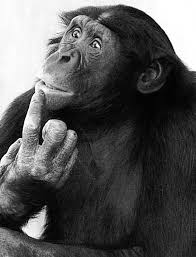
\includegraphics[width=1.in]{think.jpg}
\ecenter
上述物态变化规律能用微观模型来解释吗?
\ech
\end{frame}

\begin{frame}
\chtitle{分子力和势能的经典模型}
\bch

\bmini{0.47}
{\small
右图是一个典型的分子势能随分子间距离$r$变化的经典模型

在某“平衡距离” $r_0$ (大都为一两个\AA) 处势能最低,分子力为零。

束缚能是处于$r_0$的分子逃逸到无穷远需要消耗的能量。
$$E_B = U(\infty) - U(r_0) $$
$E_B$的强弱取决于化学键形式,一般在$\mathrm{eV}$附近几个数量级内。}
\emini
\hspace{0.2in}
\bmini{0.46}

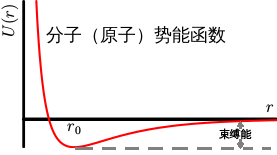
\includegraphics[width=1.8in]{atom_potential.png}

\vspace{0.05in}

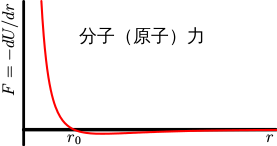
\includegraphics[width=1.8in]{atom_force.png}
\emini
\ech
\end{frame}

\begin{frame}
\chtitle{物态(State of Matter)}
\bch
物体的形态取决于分子的平均动能和束缚能的强弱比较:
\bitem
\item{{\bf 气态:平均动能 $\gg$ 束缚能}

{\scriptsize 大部分分子能够完全逃离势能的束缚成为近似的自由粒子(除了短暂的碰撞之外),分子之间的平均距离远远大于$r_0$}
}
\item{{\bf 液态:平均动能 $\sim$ 束缚能}

{\scriptsize 大部分分子能够显著地偏离平衡点,但又无法脱离势能束缚,分子之间的平均距离比$r_0$略大。}
}
\item{{\bf 固态:平均动能 $\ll$ 束缚能}

{\scriptsize 分子被束缚在势能平衡点附近很小范围内,距离几乎就是固定在$r_0$}
}
\eitem

{\scriptsize 注意:
\bitem
\item[1]{ 势能的零点可以随意选取,并且$r\rightarrow 0$时势能的变化可以远远大于束缚能的量级,所以教材上的“运动$\gg$分子力”和“动能$\gg$势能”等表述都不严谨。}
\item[2]{分子的动能包括平动,转动,以及多原子分子自己内部的振动等。显然用来逃离束缚的主要是分子的平动动能。我们在上面的讨论中没有特别指定是平动动能是因为一般其他形式动能和平动动能是同一个数量级的。}
\eitem
}
\ech
\end{frame}

\begin{frame}
\chtitle{课堂练习}
\bch
\bitem
\item[1]{试估算标准状态($0\cdeg$,$1\atm$)下气体分子之间的平均距离,并跟典型的$r_0$比较。}
\item[3]{如果物质分子量为$A$,密度为$\rho$,证明分子之间的平均距离约为
$$\left(\frac{1.66 A }{\rho / (\mathrm{g}\cdot \mathrm{cm}^{-3})}\right)^{1/3}\angstrom$$
}
\item[3]{试估算通常状态下液态水(原子量18,密度$1\SIg/\SIcm^3$)分子之间的平均距离和铁块(原子量56,密度$7.9\SIg/\SIcm^3$)分子之间的平均距离,分别跟典型的$r_0$比较。}
\eitem
\ech
\end{frame}


\begin{frame}
\bch
听上去好像很厉害的样子,but ...
\bcenter
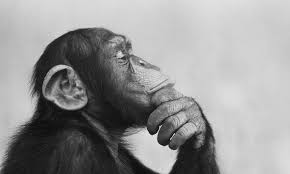
\includegraphics[width=1in]{think2.jpg}
\ecenter
既然分子势能曲线是连续光滑的,为何物态变化在宏观上有着明显的非连续性?
\ech
\end{frame}

\begin{frame}
\chtitle{整体效应}
\bch
要更完整地理解物态变化,光考虑局域的两个分子之间的相互作用是不行的,还必须考虑整体效应。
\ech
\end{frame}

\begin{frame}
\chtitle{完美的周期性结构更稳定}
\bch
哪组积木更容易推动使之发生结构变化?
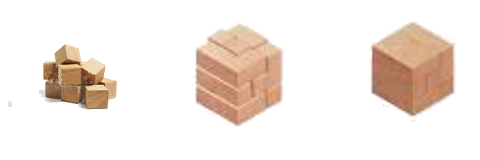
\includegraphics[width=3in]{stackcubes.png}

(A)胡乱堆砌 \ \ \ \ \  (B)不是很整齐 \ \ (C)非常整齐

\ech
\end{frame}

\begin{frame}
\chtitle{晶体 (Crystalline Solid)}
\bch
\bitem
\item{自然界大多数固体都是分子排列具有周期性的完美结构的{\bf 晶体}。完美的分子排列使得固体占据体积更小,(多分子相互作用的)总势能更低。}
\item{当我们加热固体,固体内分子的平均动能(即固体的温度)逐渐增大,到达某一临界值时,完美的分子排列结构被破坏,就发生了固态往液态的相变。这个温度临界值,叫做该物质的{\bf 熔点}。}
\item{当温度处在熔点时,虽然分子动能保持不变,破坏完美分子结构需要额外吸收能量(因为胡乱排列的分子总势能更高)。所以{\bf 晶体熔化,是一个温度不变但需要吸收能量的过程。}}
\eitem
\ech
\end{frame}

\begin{frame}
\chtitle{固液转化宏观非连续性的微观解释}
\bch
所以,对晶体而言,虽然两分子之间的势能曲线是连续的。但是多分子相互作用的总势能却会随着晶体完美的分子排列结构瓦解而有个跃变。这就是为什么宏观上固态到液态的转变有明显的非连续性。
\ech
\end{frame}

\begin{frame}
\chtitle{多晶和单晶}
\bch
\bitem
\item{晶体可以是肉眼可见的大块,有着明显的规则外形。例如水晶,金刚石等。这种晶体称为单晶。}
\item{晶体也可以是肉眼不可见,微米量级的小块晶粒组成。很多金属都是多晶。多晶有可能被拉成单晶。}
\item{纯冰一般是单晶,我们日常见到冰块很不规则,是含了杂质的缘故。}
\eitem
\ech
\end{frame}


\begin{frame}
\chtitle{晶体可能有多种对称性}
\bch
除了{\bf 空间平移对称性}以外,晶体分子排列而成的{\bf 晶格}还可能有{\bf 中心反演对称性},{\bf 镜像反演对称性}, {\bf 绕轴的$n$重旋转对称性($n=2,3,4,6$)}等。

一般来说,对称性越高,晶格越稳定,破坏晶格时需要的能量越大。

\bcenter
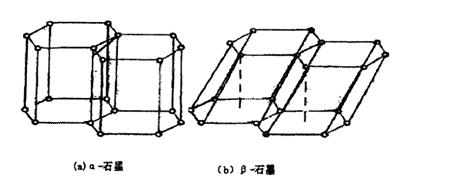
\includegraphics[width=3in]{graphite.jpg}
\ecenter

左图晶格比右图更稳定
\ech
\end{frame}


\begin{frame}
\chtitle{实际晶体可能有各种缺陷}
\bch
实际的晶体可能会有晶界(二维缺陷),位错(一维缺陷),空位或杂质(点缺陷)等。

\bcenter
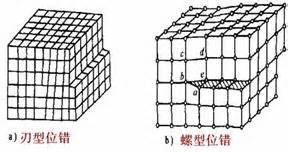
\includegraphics[width=2.5in]{solid_dislocate.jpg}
\ecenter

产生缺陷的晶体的牢固程度可能会大幅度下降。
\ech
\end{frame}


\begin{frame}
\bch
固体一定是排得整整齐齐的晶体吗?

\skiplines

未必 \bye 玻璃、松香、沥青、蜂蜡等都是{\bf 非晶体}。
\ech
\end{frame}

\begin{frame}
\chtitle{非晶体 (Amorphous Solid)}
\bch
在很小范围内非晶体的分子排列是有规则的,但“不是很整齐”。从大范围看,非晶体的分子排列方向是无序的。总结起来就是:

非晶体分子排列{\bf 短程有序而长程无序}

\skipline
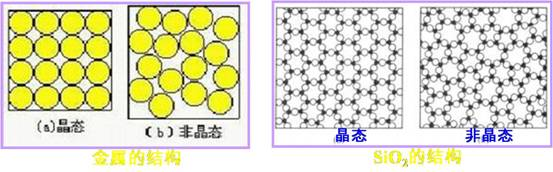
\includegraphics[width=4.3in]{amorphous_solid.jpg}

非晶体由固态向液态转变时则是各个小范围内的分子排列结构被逐渐破坏,不存在一个从完美排列到混乱排列的突变,所以非晶体熔融时温度还是在继续上升。{\bf 非晶体不存在熔点}。

\ech
\end{frame}

\begin{frame}
\bch
{\bf 液体分子排列也是短程有序长程无序},非晶体熔融为液体时又没有体积的突变,那非晶体和液体的区别在哪里呢?
\bcenter
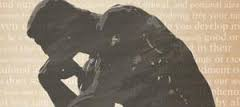
\includegraphics[width=1.5in]{think3.jpg}
\ecenter
\ech
\end{frame}

\begin{frame}
\chtitle{非晶体和液体的区别}
\bch
\bitem
\item{非晶体虽然“堆得不大整齐”,但既然为“固”体,在不发生宏观形变的情况下,其内部分子的位置是固定的。(堆得再差也是堆啊\wulian)}
\item{液体内分子并无固定位置,会发生游动,一般定居时间只有$10^{-10}s$左右。}
\eitem
\ech
\end{frame}


\begin{frame}
\chtitle{思考题}
\bch
\bcenter
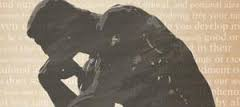
\includegraphics[width=1.5in]{think3.jpg}
\ecenter

为什么自然界中大多数物质都是晶体?
\ech

\end{frame}


\begin{frame}
\chtitle{快速淬火制作非晶体}
\bch
因为自然界中物态变化的过程都相对缓慢,物质中的分子有足够的时间“排好队”,就会形成全局能量最低态——晶体。

\skipline

如果把熔点附近的液体以极快的速度降温,使它的温度快速跨过熔点(即凝固点),并迅速降到某个比熔点更低的温度“玻璃化点”,物质中的分子没有足够的时间“排好队”,就得到“排得不那么整齐”的非晶体(局域能量最低态)。这种技术叫做“快速淬火”。几乎所有物质都可以通过这种方法人工制成非晶体。

\ech

\end{frame}


\begin{frame}
\bch
解决了固体熔化的问题,下面我们考虑液体汽化。
\ech
\end{frame}

\begin{frame}
\chtitle{汽化的宏观非连续性的微观解释}
\bch
\bitem
\item{液体内的分子虽然有较大的活动空间,但还是被周围的分子势能所束缚,做着无规则的振荡(一般在同一位置可以振荡10-100次左右)。}
\item{当我们加热液体,液体分子的平均动能(即液体的温度)逐渐增大,到达某一临界值时,分子就挣脱了势能的束缚变为在容器内到处飞行的近自由粒子(除短暂的碰撞,几乎不受力)。}
\item{虽然从两分子之间的势能曲线来看这是一个连续的过程(从几乎逃逸到逃逸),但多分子相互作用的整体效应仍不可忽略。分子大都成为自由粒子之后,原先液体的聚团特性立刻被破坏,又一次造成总体势能的跃变。所以{\bf 液体汽化也是一个温度不变但需要吸收能量的过程}。}
\eitem
\ech
\end{frame}

\begin{frame}
\chtitle{外界压强的影响}
\bch
\bitem
\item{前面的讨论忽略了外界环境的影响,实际上无论是熔化还是汽化,大部分物体的体积都会突然增大,在固定压强下体积增大就会对外界做功,需要消耗额外的能量。外界压强越大,做的功越大。所以大部分物质的熔点,沸点和潜热都随着压强增加而增加。

\scriptsize 注: 冰的熔化过程比较特殊,它的体积在这个过程中减小(微观原因和特殊的化学键有关,我们之后再讨论),所以熔点和熔化热反而随着压强增大而减小。}
\item{由于固液态的体积变化不大,所以压强对熔点和熔化热的影响不显著。}
\item{汽化过程的体积增大是非常显著的(一般体积要增大三个数量级左右),在标准大气压下做的功往往跟总体分子势能的变化的数量级接近,属于不可忽略的效应,所以沸点和汽化热对压强的依赖性很显著。}
\eitem
\ech
\end{frame}

\begin{frame}
\chtitle{思考题}
\bch
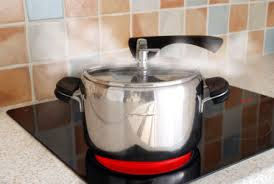
\includegraphics[width=1.5in]{gaoyaguo.jpg}

\includegraphics[width=1.5in]{dunzhuti.jpg}

为什么高压锅炖猪蹄炖得更软?
\ech
\end{frame}


\begin{frame}
\chtitle{思考题}
\bch
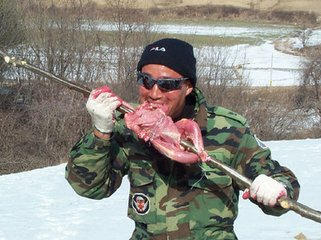
\includegraphics[width=2in]{eatraw.jpg}

在线等,急!为什么在西藏煮东西煮不熟?(\wulian你确定这煮过了?)
\ech
\end{frame}

\begin{frame}
\chtitle{很炫的小学生题目}
\bch
考虑物质汽化时气液共存的状态,设在沸点该物质每$\SImol$液态的体积为$V_L^{\rm mol}$,每$\SImol$气态的体积为$V_G^{\rm mol}$,则该物质的液态共存时每$\SImol$体积为
$$\bar{V} = V_L^{\rm mol} x_L + V_G^{\rm mol} x_G$$ 
其中$x_L$, $x_G$分别为液,气态的摩尔分数,$x_G + x_L = 1$。由此即有
$$x_G = \frac{\bar{V} - V_L^{\rm mol}}{V_G^{\rm mol} - V_L^{\rm mol}},\ x_G = \frac{V_G^{\rm mol} - \bar{V}  }{V_G^{\rm mol} - V_L^{\rm mol}}$$

虽然看起来像小学生题目,教材中它有个很炫的名字:{\bf 气液共存的杠杆法则}
\ech
\end{frame}

\begin{frame}
\chtitle{闭合系的$p$-$V$-$T$曲面($p$-$V$-$T$ diagram)}
\bch
\bitem
\item{下面我们要把讨论范围扩展到极端温度或者极端压强等非普通条件。为此我们必须把实验条件精确化:考虑{\bf 封闭且处于热平衡的单一成分物质}。}
\item{
\bmini{0.5}跟理想气体类似,物质的三个{\bf 状态参量}:压强$p$,体积$V$和热力学温度$T$并不互相独立,而是满足一定的函数关系。在以$p$, $V$, $T$为三条坐标轴的直角坐标系里,物质的状态参量$(p, V, T)$对应的点只能在一个曲面上,称为该物质的{\bf $p$-$V$-$T$曲面}。
\emini
\bmini{0.46}
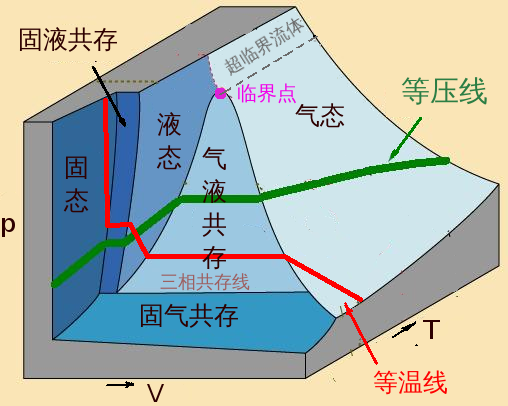
\includegraphics[width = 1.5in]{PVTdiagram.png}
\emini
}
\eitem
\ech
\end{frame}

\begin{frame}
\chtitle{典型的等压线和等温线}
\bch
\bmini{0.6}
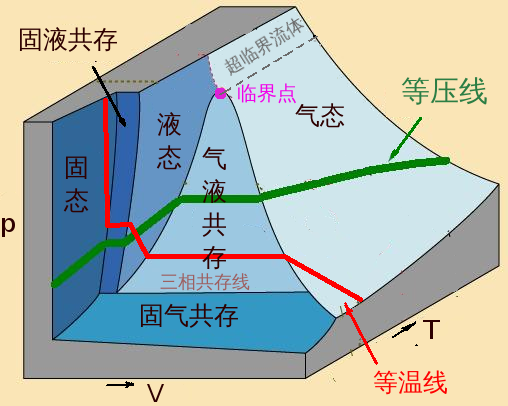
\includegraphics[width = 2.6in]{PVTdiagram.png}
\emini
\bmini{0.36}
{\small

\bitem
\item{典型的等压(加热)线:

 固态升温$\rightarrow$恒温熔化$\rightarrow$液态升温$\rightarrow$恒温汽化$\rightarrow$气态升温}

\item{典型的等温(压缩)线:

气态升压$\rightarrow$恒压液化$\rightarrow$液态升压$\rightarrow$恒压凝固$\rightarrow$固态升压

}
\eitem
}
\emini
\ech
\end{frame}


\begin{frame}
\chtitle{临界点}
\bch
\bitem
\item{\small 当我们逐步增加等温线的温度,气液共存线逐渐变短,直到缩为一个{\bf 临界点}。临界点的温度称为{\bf 临界温度$T_K$}。在温度为$T_K$的等温线上,液态和气态之间连续转化(没有体积跃变),且临界点为一个拐点,数学上即}
\eitem
\bmini{0.55}
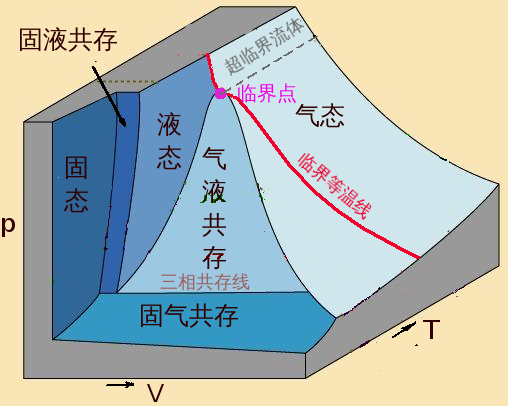
\includegraphics[width = 2.2in]{PVTdiagram_TK.png}
\emini
\bmini{0.4}
{\small
$$\left(\frac{d p}{d V}\right)_{T=T_K} = \left(\frac{d^2 p}{d V^2}\right)_{T=T_K} = 0$$ 
\bitem
\item{$T>T_K$的等温线都是气态{\scriptsize(教材把超临界流体归类为气体,实际它也有部分液体性质)},所以在$T_K$以上不能通过等温压缩得到液态。}
\eitem
}
\emini
\ech
\end{frame}

\begin{frame}
\chtitle{三相共存线和三相点}
\bch
\bitem
\item{\small 当我们逐步减小等温线的温度,固液共存段和气液共存段的差别逐步减小,直到两者合并为一条线,即三相共存线。}
\eitem
\bmini{0.6}
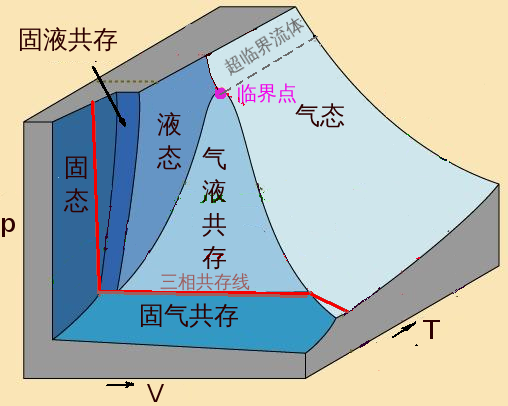
\includegraphics[width = 2.6in]{PVTdiagram_T3.png}
\emini
\bmini{0.36}
{\small
\bitem
\item{当物质沿着三相共存线变化时,固液气三态并存,体积(以及三态物质的比例)发生变化,压强和温度都不变。}
\item{三相共存线对应的温度称为{\bf 三相点$\Tthree$}。按定义,水的三相点为$273.16\SIK$。}
\eitem
}
\emini
\ech
\end{frame}

\begin{frame}
\chtitle{$p$-$T$三相图}
\bch
\bmini{0.63}
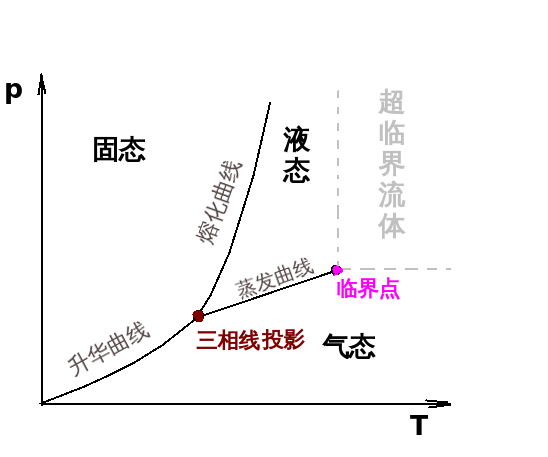
\includegraphics[width = 2.6in]{PTdiagram.png}
\emini
\bmini{0.32}
{\small
把$p$-$V$-$T$曲面投影到$p$-$T$平面上,得到$p$-$T$三相图(也叫气液固三相图),可以很清楚地看出三相点不依赖于压强和体积。

从蒸发曲线上还可以直接读出{\bf 饱和蒸气压}(即气液共存时的压强)随温度的变化。}
\emini
\ech
\end{frame}


\begin{frame}
\chtitle{还没有凌乱吗?}
\bch
意犹未尽的学霸们必须思考一些更深奥的问题

\bcenter
\bmini{0.5}

\includegraphics[width=2in]{think4.jpg}

让暴风雨来得更猛烈些吧
\emini
\ecenter
\ech
\end{frame}


\begin{frame}
\chtitle{进阶知识I:道尔顿分压定律}
\bch
纯净的气体并不容易获得,实验中我们往往得到的是混合气体(例如由排水法收集的气体里混合了饱和水蒸气)。对混合气体有著名的{\bf 道尔顿分压定律:混合气体的压强等于各组分的分压强之和。}

\skipline

对于理想气体,这是很容易理解的:各组分的气体分子虽然会发生碰撞,但因为已经达到了化学平衡和热平衡,各组分气体分子的速度和位置分布密度不因碰撞而发生改变。按照上节课我们对理想气体压强的推导(也可参考教材第28页),每种气体对压强都有$\frac{1}{3}\overline{\veccalp\cdot\vecv}$ 的独立贡献。

\skipline

对于实际气体,道尔顿分压定律并非严格的定律,但往往是很好的近似。
\ech
\end{frame}


\begin{frame}
\chtitle{思考题}
\bch
空气的平均分子量为29,试计算标准状态下($1\atm, 0\cdeg$)空气的密度。
\ech
\end{frame}

\begin{frame}
\chtitle{相对论气体的压强(本页内容仅供娱乐)}
\bch
{\small
如果气体分子的运动接近光速$\upsilon \approx c$,则分子能量为$\varepsilon = \sqrt{\calp^2c^2 + m^2}\approx \calp c$。
压强
$$ p = \frac{1}{3}n \overline{\calp\cdot \vecv} \approx \frac{1}{3} n \bar{\varepsilon}$$
这跟非相对论气体$p = \frac{2}{3}n \bar{\varepsilon}$差别了一个因子2。

如果是静质量为零的气体$m=0$,上述结论就是严格的,且气体的能量密度可以写成$\rho = n\bar{\varepsilon}$。我们即得到光子气体的状态方程:
$$p = \frac{1}{3}\rho$$
}
{\darkblue \scriptsize 脑洞大开:在广义相对论里,很多时候我们可以用能量动量张量的迹$(\rho + 3p)/c^2$来代替牛顿万有引力公式里的质量密度(这是我编的,正式场合慎用)。
\bitem
\item{\darkblue  因为光子气体的$3p = \rho$,考虑压强修正算出来的光线偏折角是不考虑压强修正时的计算结果的两倍,历史上著名的广义相对论的星光偏折实验就是在验证这个因子2。}
\item{\darkblue  在现代宇宙学里的暗能量是压强$ p \approx -\rho$的模型,于是$\rho + 3p = -2\rho <0$,产生了“负引力”,导致宇宙加速膨胀。}
\eitem
}
\ech
\end{frame}

\begin{frame}
\chtitle{进阶知识II:实际气体的范德瓦尔斯方程(van der Waals Equation of State)}
\bch
范德瓦尔斯方程是对理想气体状态方程$pV = \nu RT$的修正:
\bitem
\item{理想气体模型假设分子大小为零,实际气体的分子是要占据一定体积的。假设{\bf 每$\SImol$分子占据的体积为$b$},气体摩尔数为$\nu$,则容器的有效空间体积为
\bmini{0.47}
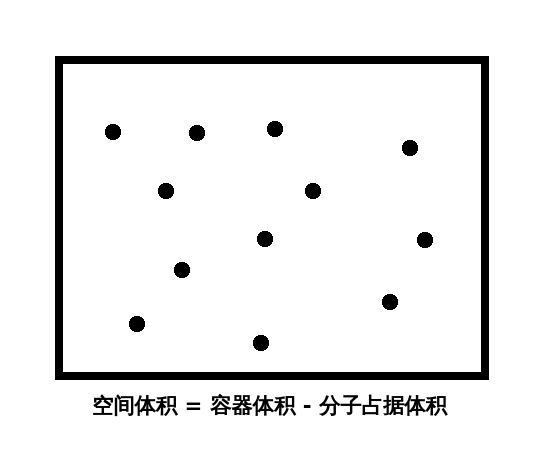
\includegraphics[width= 2in]{Vspaceeff.png}
\emini
\bmini{0.47}
$$ V_{\rm eff} = V - \nu b$$

\skipline

我发现物理书里写乘积的顺序很有讲究,例如$\nu b$(大声读一遍…)
\emini
}
\eitem
\ech
\end{frame}




\begin{frame}
\chtitle{范德瓦尔斯方程(续):分子力修正}
\bch
\bitem
\item{\small 理想气体模型假设分子之间无作用力,分子的运动产生{\bf 动理压强},记为$p_k$。实际气体的分子有微弱的长程吸引力,产生{\bf 内压强},记为$p_U$。
假设长程分子力有效距离为$L$,{\bf 单位$\SImol$分子对有效距离内的单位$\SImol$分子的平均吸引力为$a/L^4$}。如图,考虑面积为$dS$,厚度为$L$的紧贴在一起的气体薄层A和B之间的作用力。我们把A和B都划分成$dS/L^2$个边长为$L^3$的小方块,并粗略地认为只有紧挨的小方块对之间才有吸引力。那么总吸引力为}
\eitem
\bmini{0.28}
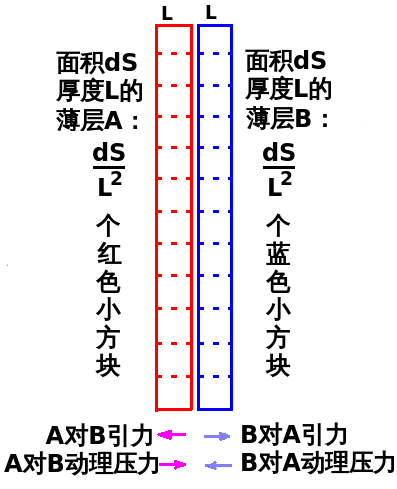
\includegraphics[width=1.2in]{PUrealgas.png}
\emini
\bmini{0.7}
{\small  
$$ \frac{a}{L^4}\left(\frac{L^3}{V}\nu\right)^2 \frac{dS}{L^2} = a \left(\frac{\nu}{V}\right)^2 dS$$
显然内压强和动理压强符号相反,故内压强为 $p_U = - a(\nu/V)^2$,在总压强中剔除它的贡献,即得动理压强
$$p_k = p - p_U = p + \frac{\nu^2 a}{V^2}$$
}
\emini
\ech
\end{frame}

\begin{frame}
\chtitle{范德瓦尔斯方程(续):结论}
\bch
假设考虑了分子大小和分子力修正之后的空间体积$V_{\rm eff}$和动理压强$p_k$仍满足理想气体的状态方程,即得{\bf 范德瓦尔斯方程}:
$$ \left(p+\frac{\nu^2 a}{V^2}\right)\left(V - \nu b\right) = \nu R T$$

跟理想气体状态方程比较,范德瓦尔斯方程更精确地描述了实际气体,但它仍然只是一个近似方程。
\ech
\end{frame}


\begin{frame}
\chtitle{范德瓦尔斯方程的应用举例(该内容仅供娱乐)}
\bch
{\small 
我们用范德瓦尔斯方程来求解课本习题1-2,设定体温度计内气体体积为$V$,三次测量时气体的单位体积摩尔数分别为$x_1$, $x_2$, $x_3$。设待测温度为$T$,由范德瓦尔斯方程
\bea
500\SImmHg + a x_1^2 &=& \frac{x_1 R\Tthree}{1 - bx_1},\ 734\SImmHg + a x_1^2 = \frac{x_1 R T}{1 - bx_1}\newl
200\SImmHg + a x_2^2 &=& \frac{x_2 R\Tthree}{1 - bx_2},\  293.4\SImmHg + a x_2^2 = \frac{x_2 R T}{1 - bx_2}\newl
100\SImmHg + a x_3^2 &=& \frac{x_3 R\Tthree}{1 - bx_3},\  146.68\SImmHg + a x_3^2 = \frac{x_3 RT}{1- bx_3}
\eea
由于$R$和$\Tthree$是已知的,一共有六个方程和六个未知数,数值求解得到$T\approx 400.628\SIK$,但是,解出来的$b<0$,跟我们最初推导范德瓦尔斯方程的假设不符。如果强行要求$b>0$,并取误差最小的点作为近似解,则得到$T \approx 400.584\SIK$,这个结果就和用最小二乘法推出来的结果($400.575\SIK$)相近了。
}
\ech
\end{frame}



\begin{frame}
\chtitle{技能回顾:最小二乘法(\bye学霸请自动跳过)}
\bch
{\scriptsize
课本习题1-2的最小二乘法计算细节:已知数据点为
\bea
(p_1, T_1) &=&  (734 \SImmHg, \frac{734}{500}\times 273.16 \SIK) = (734\SImmHg, 400.999\SIK) \newl
(p_2, T_2) &=&  (293.4 \SImmHg, \frac{293.4}{200}\times 273.16 \SIK) = (293.4\SImmHg, 400.726\SIK) \newl
(p_3, T_3) &=&  (146.68\SImmHg, \frac{146.68}{100}\times 273.16\SIK) = (146.68\SImmHg, 400.671\SIK)
\eea
求平均,并每个数据点减去平均:
\bea
(\bar{p},\bar{T}) &=& \left(\frac{p_1+p_2+p_3}{3},\frac{T_1+T_2+T_3}{3}\right) = (391.36\SImmHg, 400.799\SIK) \newl
(\Delta p_1, \Delta T_1) &=& (p_1-\bar{p}, T_1-\bar{T})=(342.64 \SImmHg, 0.200\SIK), \newl
(\Delta p_2, \Delta T_2) &=& (p_2-\bar{p}, T_2-\bar{T})= (-97.96 \SImmHg, -0.073\SIK), \newl
(\Delta p_3, \Delta T_3) &=& (p_3-\bar{p}, T_3-\bar{T})= (-244.68 \SImmHg, -0.128\SIK)
\eea
设拟合直线为$T = kp + b$,则
\be
k = \frac{\sum \Delta p \Delta T}{\sum \Delta p^2}= 0.0005726 \SImmHg/\SIK, \ b = \bar{T} - k\bar{p} = 400.575 \SIK
\ee
所以外推到$p=0$时$T = b = 400.575\SIK$,这就是所求的温度。
}
\ech
\end{frame}


\begin{frame}
\chtitle{计算实际气体的临界温度$T_K$ (该内容仅供娱乐)}
\bch
范德瓦尔斯方程可以写成
$$ p = \frac{\nu R T}{V - \nu b} - \frac{\nu^2 a}{V^2}$$
根据前述临界温度的条件
$$\left(\frac{d p}{d V}\right)_{T=T_K} = \left(\frac{d^2 p}{d V^2}\right)_{T=T_K} = 0$$ 
即得
\bea
T_K &=& \frac{8 a}{27 Rb} \newl
V_K &=& 3\nu b \newl
p_K &=& \frac{a}{27 b^2} 
\eea
由此得到“临界系数” $K = \frac{\nu RT_K}{p_K V_K} = 2.667$,实际物质的临界系数并非常数,大约为3到4之间。
\ech
\end{frame}


\begin{frame}
\chtitle{对应态方程 (该内容仅供娱乐)}
\bch
可以用临界点的温度,压强和体积为单位把范德瓦尔斯方程无量纲化。定义

对应温度$\tau = T/T_K$, 

对应体积$\omega = V/V_K$,

对应压强$\pi = p/p_K$,

就得到对应态方程
$$\left(\pi + \frac{3}{\omega^2} \right)(3\omega - 1) = 8\tau$$

\ech
\end{frame}

\begin{frame}
\chtitle{位力展开(该内容仅供娱乐)}
\bch
我们考虑用理想气体状态方程得到的压强$p$乘一个修正因子的方法来描述实际气体。

把这个修正因子对$\frac{\nu}{V}$(因为$\frac{\nu}{V}$代表了气体的稀薄程度)进行泰勒展开:
$$p = \frac{\nu RT}{V}\left[1+ \frac{\nu}{V}B(T) + \frac{\nu}{V}C(T) + \ldots \right]$$
$B(T)$(又可以大声读了…)和$C(T)$称为第二和第三位力系数。

\skipline

把范德瓦尔斯方程进行级数展开并进行对比可以得到
$$B(T) = b - \frac{a}{RT}, \ C(T) = b^2$$

在“波意耳”温度$T_B = \frac{a}{Rb} = \frac{27}{8}T_K$,第二位力系数消失,这时物态方程与波意耳定律偏离最小。
\ech
\end{frame}



\begin{frame}
\chtitle{进阶知识III:液体的压强}
\bch
实际气体的内压强是对动理压强的一个小修正。我们还记得内压强和分子数密度的平方成正比。液体内分子数密度要比气体高三个数量级左右,所以内压强要大很多。一般情况下,{\bf 液体的内压强和动理压强差不多大,两者符号相反而几乎抵消,导致总压强(教材中称为“外压强”)要小一个多数量级。}
$$ |p_k + p_U| \ll |p_U|\approx |p_k|$$
当然,这只是液体平均动能$\sim$束缚能 的另一种表现。
\ech
\end{frame}

\begin{frame}
\chtitle{进阶知识IV:液体表面张力}
\bch
 液体表面是不对称的,如果液体处处分子数密度一样的话,“内部分子扩散到表面”要难于“表面分子扩散到内部”,因为前者需要克服较大的分子引力。这种分子扩散不平衡会导致更多表面分子跑到内部去。当达到{\bf 扩散平衡时,液体表面分子数密度比内部小。} 

\skipline

表面分子之间偏离平衡点的距离增大,就好像弹簧被拉长了一样(但还未拉断弹簧成为气体),造成了切向的(即沿着液体表面试图使液体表面积减小的){\bf 张力}。这就又需要额外的力学平衡(通常表现为液体表面弯曲且内外压强不等)。

\ech
\end{frame}

\begin{frame}
\chtitle{进阶知识V:化学键}
\bch
经典的分子势能模型并不十分准确,而完整精确的量子描述我们由于还未学习量子力学而无法理解,介于量子模型和经典模型之间的唯象模型就是{\bf 化学键}(高中化学课的痛苦回忆纷纷涌上心头\wulian)。

\skipline

{\bf 经典模型中的束缚能的大小和化学键的强弱密切相关。强的化学键有离子键,共价键和金属键,负责把原子和原子结合成分子或晶体。弱的化学键有范德瓦尔斯键和氢键,负责把分子和分子结合成晶体。}
\ech
\end{frame}

\begin{frame}
\chtitle{离子键}
\bch

例如NaCl,Na失去一个电子而带正电,Cl得到一个电子而带负电。离子(Na$^+$和Cl$^{-}$)之间的静电吸引力使它们结合在一起,成为晶体。这种{\bf 将正负离子结合起来的静电力称为离子键}。

\skipline

\bcenter
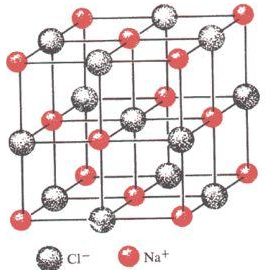
\includegraphics[width=1.5in]{NaCl.png}
\ecenter

\ech
\end{frame}

\begin{frame}
\chtitle{共价健 }
\bch

{\bf 共价键是两个原子共享价电子形成的} (“共享”的原理涉及量子力学,我们先呵呵\bye)。

\skiplines

共价键和离子健对应的束缚能都是$\sim 100 \SIkJ/\SImol$的数量级。氧气$O_2$的共价键$O=O$强度约为$120 \SIkcal/\SImol$,在燃烧反应中,仅考虑氧气的$O=O$断裂释放出的能量,忽略其他发生变化的键的能量,可以粗略估算燃烧释放的热量(见教材例题5和思考题1-16, 1-17)。
\ech
\end{frame}

\begin{frame}
\chtitle{金属键}
\bch

{\bf 金属键是通过把所有外层电子共有化形成的}

\skipline

靠离子键结合的晶体的晶格如果滑移奇数格,静电引力变斥力,就容易发生碎裂。(例如食盐很容易敲碎)

\skipline

靠金属键结合的晶体的晶格即使发生滑移,共有化的电子仍然起着“粘合剂”的作用,就不容易发生碎裂。所以金属一般有很好的延展性。

\ech
\end{frame}

\begin{frame}
\chtitle{范德瓦尔斯键}
\bch

中性分子之间是怎么吸引的呢?

\skipline

中性分子内正负电荷可以产生微小的分离而产生电偶极子。{\bf 范德瓦尔斯键就是中性电偶极子之间的吸引力},一般比较弱,为1-10$\SIkcal/\SImol$的数量级。
\ech
\end{frame}

\begin{frame}
\chtitle{氢键 (本页内容仅供娱乐)}
\bch
氢是一种比较特殊的元素,它只有一个电子,所以形成共价键时,氢原子的电偶极性比较明显,可以通过范德瓦尔斯键和另一原子结合,这种特殊的范德瓦尔斯键称为氢键。

\skipline


冰和接近$0\cdeg$的水里有很多氢键,随着温度升高氢键被破坏而变得越来越少。氢键使得水分子容易排列成空旷的六角晶格,所以氢键越多,体积越大。随着温度升高氢键断裂,体积变小。
这个效应和热胀冷缩效应相互竞争,导致了水在$4\cdeg$以下热缩冷胀的奇特性质。


\ech
\end{frame}


\begin{frame}
\chtitle{第二周作业(编号续第一周作业1.-3.)}
\bch
\bitem
\item[4]{一碗米饭大概含有$300\SIkcal$的热量,试估算这些能量能够把一个体重$60\SIkg$的人举到多高。}
\item[5]{日常环境下,水银的比热是$139 \SIJ/(\SIkg\cdot\SIK)$,密度是$13.6\SIg/\SIcm^3$。请问同体积的水银和水哪个升高$1\cdeg$需要的吸收热量更多?}
\item[6]{教材习题1-16}
\eitem
\ech
\end{frame}


\end{document}
